\section{Simulated Model}


\subsection{Simulation}

The modelling of the system in a virtual environment is an important step to
allow experiments to be done in a simulator. The simulated experiments can be
replicated and repeated more easily, providing more data to analysis of the
applied algorithms. Most algorithms used in autonomous robotic navigation is
dependant on fine tuned parameters to fit the needs of the application in case.
With simulations these parameters and its effects can be better understood and
be set more closely to the desired ones in the real scenario. Also, the
simulation environment gives the ability to more researches to test the platform
and conduct experiments of each system component at the same time independently
with the results being more easily exchanged.

With this concerns in mind, the CaRINA platform was modelled to be simulated in
Gazebo, a physics simulator provided in ROS environment. There are othes 3D
simulatos that is somehow integrated with ROS, but Gazebo is more tightly closed
and is designed with ROS in mind, so, is the native choice when working with
ROS. Actually, its physics simulation is based on ODE and provides only ridgid
body dynamics, but others physical simularion libraries like Bullet and Simbody
are being integrated to provide a broader range of simulations and physics
dynamics. Since our main purpose is to check and avoid collisions the currently
physical simulation dynamics available in Gazebo is suitable for our
experiments. One example of the model in Gazebo in a simulated unstrucured
scenario can be seen in \fig{fig:gazebo}. The model in \fig{fig:model} is
presented in the ROS visualization tool called RViz.


\begin{figure}[h!]
	\begin{minipage}[b]{1\linewidth}
	    \centering
	    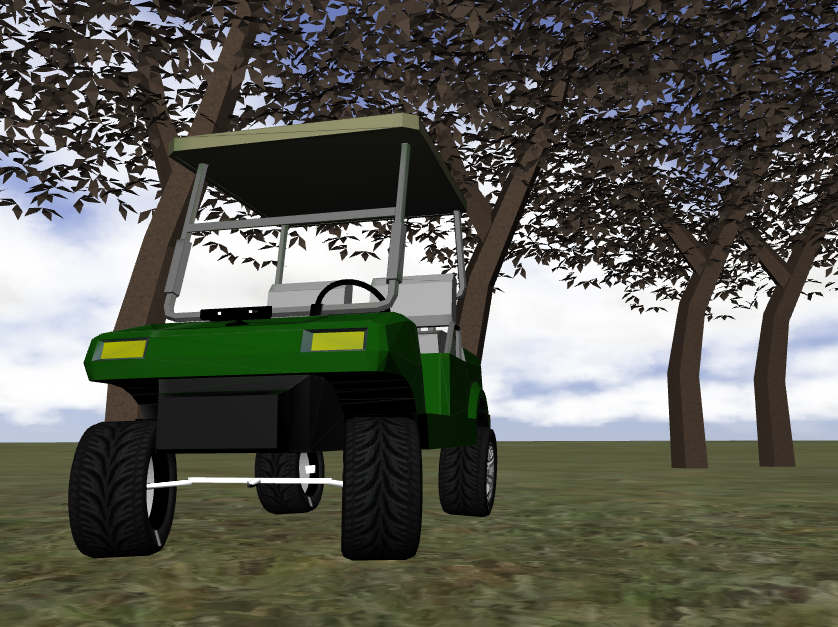
\includegraphics[width=8cm]{modelo_carina/carina_gazebo_frente_fundo.png}
	 	\caption{CaRINA I model on unstructured scenario in Gazebo simulator}
	 	\label{fig:gazebo}
	\end{minipage}
\end{figure}


\begin{figure}[ht]
	\begin{minipage}[b]{1\linewidth}
	    \centering
	    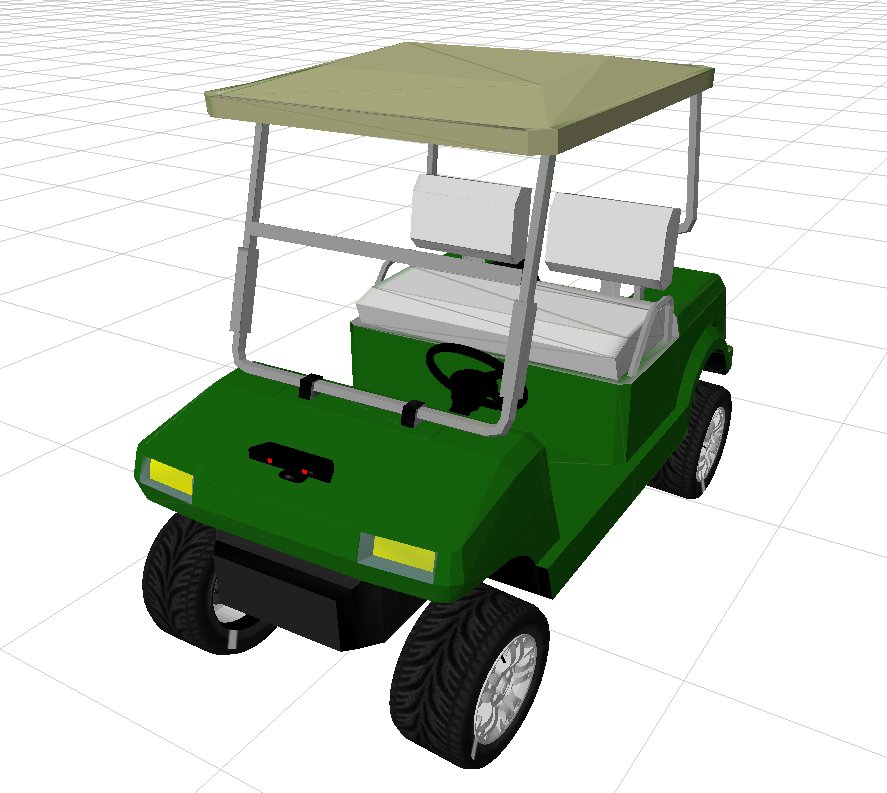
\includegraphics[width=8cm]{modelo_carina/carina_rviz_fundo_branco.png}
	 	\caption{CaRINA I virtual model}
	 	\label{fig:model}
	\end{minipage}
\end{figure}


\subsection{Model Description}

For modelling robots in ROS there is a formal description languange called URDF.
URDF is a language in XML formatting that is used basically to describe the
transform relations between the robot's coordinates frames. Each moving part of
the robot and each sensor has its own reference coordinate frame for the
generated data. In ROS, all coordinate systems are kept by a component called TF
that is responsible to provide the transformed coordinates from one frame to
another. This is an important concept and framework provided by ROS, where data
can be generated and manipulated within its own fixed coordinate frame and then
transformed easily to others coordinates frames for combining sensors data and
robot states. Since these transforms must be done from one frame to another,
uniquely and in any order, the robot coordinates frames are represented by a
tree in a parent-child relation (\fig{fig:tf},\fig{fig:tree}).

\begin{figure}[h!]
	\begin{minipage}[b]{0.5\linewidth}
	    \centering
	    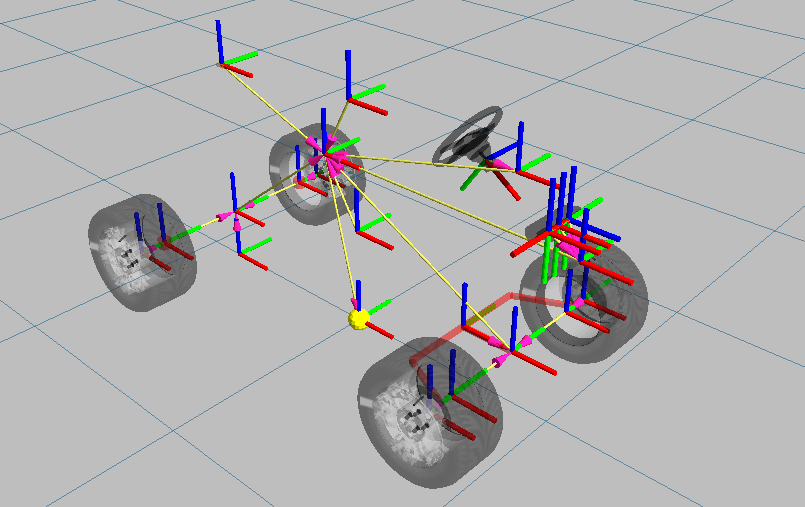
\includegraphics[width=6cm]{modelo_carina/carina_tf_side_wheels_transp.png}
	 	\caption{Transform frames (TF) reference cooridnates}
	 	\label{fig:tf}
	\end{minipage}
	\begin{minipage}[b]{0.5\linewidth}
	    \centering
	    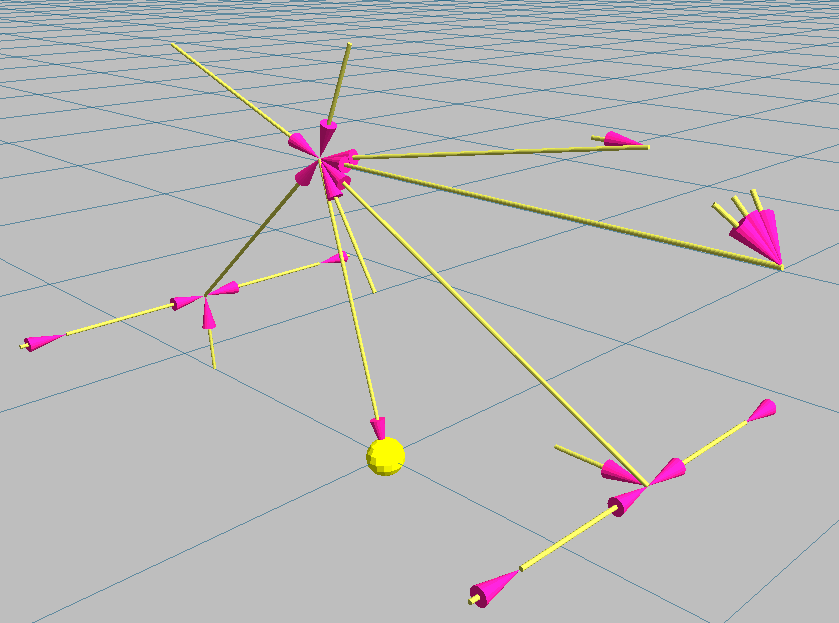
\includegraphics[width=6cm]{modelo_carina/carina_tf_side_no_axis.png}
	 	\caption{Tree representation}
	 	\label{fig:tree}
	\end{minipage}	
\end{figure}

Most physical simulation libraries uses the concept of links and joints
to describe physical relations of the structures of a body. A joint describe
a relation between links and both can present physical properties like friction
coefficients, elasticity and masses. These links and joint represent physical
relations and mechanical structures of the robot like arms, wheels and its
axels and so on. To describe links and joints relations, a graph representation
would be more suited and this makes the URDF tree structure a little limiting
to fully describe the model.

Gazebo has its own XML description language called SDF to model scenarios and
robots with its physics parameters. SDF share some compatibility with URDF and
URDF can be extended with Gazebo specific tags, this way the same robot
description can be shared between ROS and Gazebo. The Gazebo specific modelling
descriptions are used to plug sensors and controllers to the virtual model and
also allows describing some mechanical restrictions not permited by the tree
structure of URDF, like the case in the CaRINA model where the Ackermann
Geometry was modelled (\fig{fig:ackermann}).

\begin{figure}[h!]
	\begin{minipage}[b]{1\linewidth}
	    \centering
	    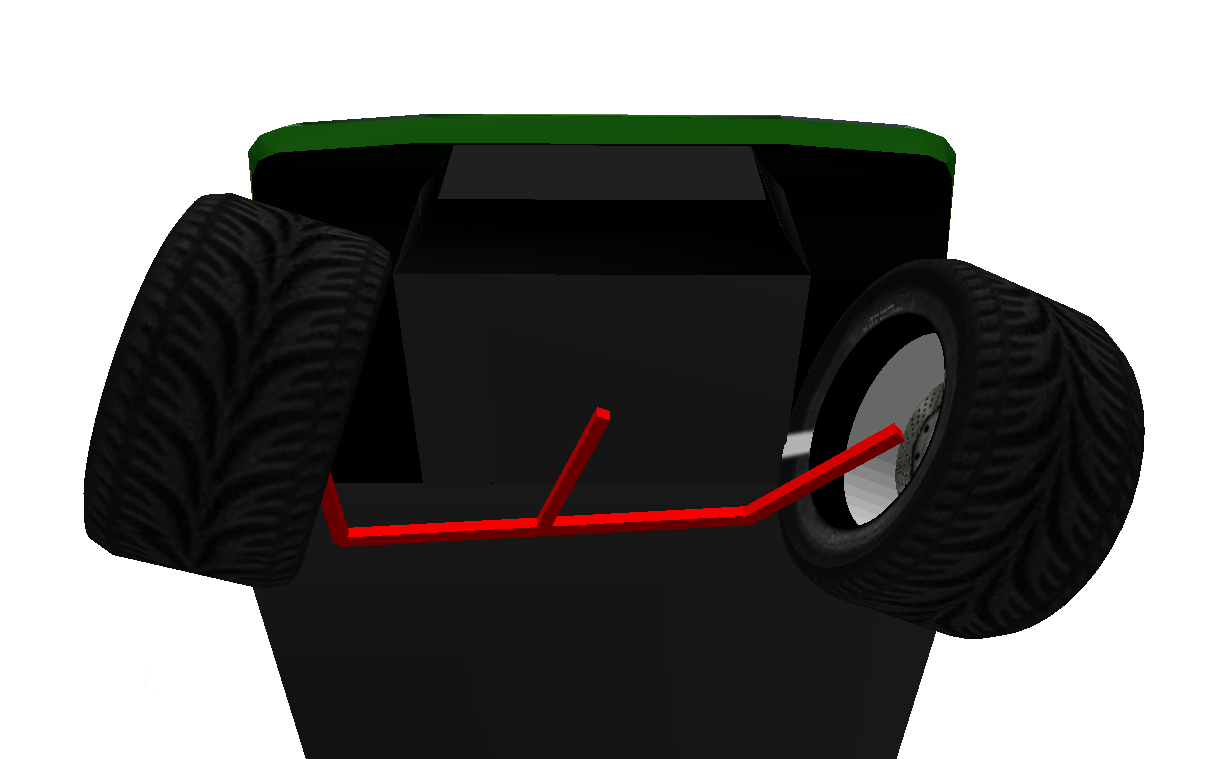
\includegraphics[width=6cm]{modelo_carina/carina_rviz_steering.png}
	 	\caption{Ackermann steering geometry modelled in simulation}
	 	\label{fig:ackermann}
	\end{minipage}
\end{figure}

We also put on the virtual model a suspension mechanism independant on each
wheel. Since our intentions are not to simulate the mechanical behaviour of the
car itself but our autonomous navigation systems, the suspension is an
aproximation model just enought to enable us to simulate on uneven terrains
avoiding the kicking collision effect with the ground caused by the ridgid body
physics simulation and keeping the four wheels in contact with the ground to
avoid loss of traction, splipages and unstable poses of the vehicle that
diverges from real situations. One other effect desired from the simulated
suspension is the balancing of the vehicle when bending, accelareting and
breaking, that will have a direct effect on the sensors reading and be more
close to real situations. This give us a better simulated IMU data with a more
realistic associated noise (\fig{fig:uneven}).

\begin{figure}[ht]
	\begin{minipage}[b]{1\linewidth}
	    \centering
	    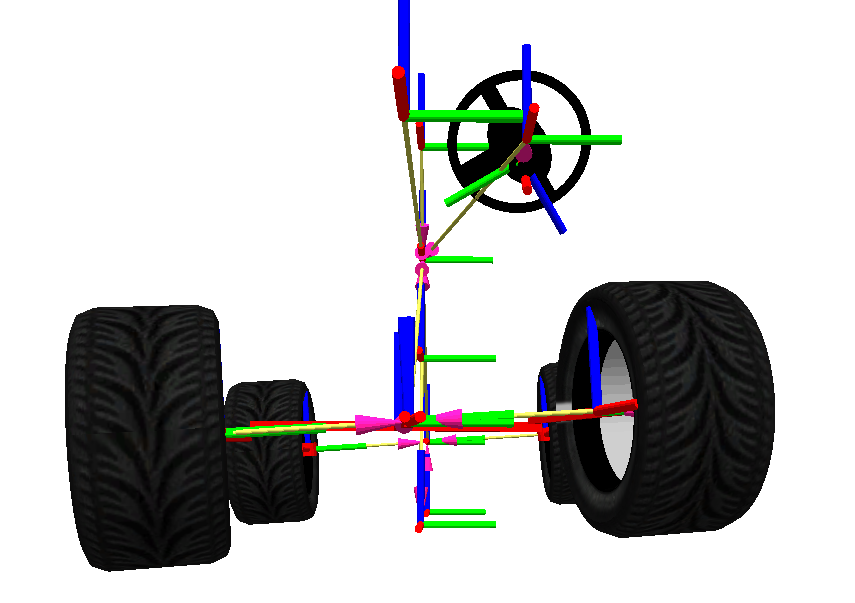
\includegraphics[width=8cm]{modelo_carina/carina_rviz_uneven_susp.png}
	 	\caption{Suspension effect on an uneven terrain}
	 	\label{fig:uneven}
	\end{minipage}
\end{figure}



 

